\documentclass[12pt, oneside]{article}   	% use "amsart" instead of "article" for AMSLaTeX format
\usepackage{color}
\usepackage{geometry}                		% See geometry.pdf to learn the layout options. There are lots.
\geometry{letterpaper}                   		% ... or a4paper or a5paper or ... 
%\geometry{landscape}                		% Activate for for rotated page geometry
%\usepackage[parfill]{parskip}    		% Activate to begin paragraphs with an empty line rather than an indent
\usepackage{graphicx}				% Use pdf, png, jpg, or eps§ with pdflatex; use eps in DVI mode
								% TeX will automatically convert eps --> pdf in pdflatex		
\usepackage{amssymb}
\usepackage{amsmath}
\usepackage[compact]{titlesec}
\linespread{1.7}
\usepackage{float}
\usepackage{pdflscape}
%\usepackage{rotating}
\usepackage{soul}
%\usepackage{longtable}
%\usepackage{threeparttable}
%\usepackage{lineno}
\usepackage[round]{natbib} %round makes pare{}ntheses instead of square brackets
\usepackage{url}
%\usepackage{authblk}
\setcounter{secnumdepth}{4}
\titleformat{\paragraph}
{\normalfont\normalsize\bfseries}{\theparagraph}{1em}{}
\titlespacing*{\paragraph}
{0pt}{3.25ex plus 1ex minus .2ex}{1.5ex plus .2ex}
\graphicspath{ {images/} }

\title{Clownfish metapopulation persistence draft}

\begin{document}
\date{}
\maketitle{}

%\section*{Abstract}

\section*{Introduction}

Paragraph 1: Long been a challenge to understand how marine metapopulations - patchy, interconnected populations - are connected and how they persist. Particularly challenging in the marine environment, where much movement happens at the larval stage - high mortality, hard to tag/track, can go far b/c of currents. Of key interest, though - both just because we want to understand population dynamics, persistence, and connectivity for basic ecological reasons, and for more applied reasons, like conservation (establishment of marine protected areas), understanding where to fish.

Lots of theory has been developed about how we would expect populations largely connected by larval movement to persist, which essentially boils down to replacement. To understand persistence, we need to know 1) whether we see replacement and 2) the origins of that replacement - self or other patches? Define and distinguish self persistence vs network persistence. Hastings and Botsford 2006 papers, Bostford 2009, some of the White papers (2010?), Burgess et al. 2014. Walk through the theory, our expectations for persistence, and what we need to know. Might take more than one paragraph. 

Testing/validating/demonstrating that theory empirically has been challenging but new technologies in tagging and genetics are making it more feasible. There have been some recent successes. Cite Johnson et al., Salles et al. the recent paper by someone Will works with (Garavelli or something?). Go through (briefly) what they did and found.

We continue this work with our long-ish term data set of clownfish. Like Salles (check) and Johnson (check), we use a tropical reef species blablalbah (maybe study system description goes in next paragraph). Talk about how we have longer-term data set (check that this is actually true...) so we can capture longer-term replacement, smooth out some of the year-to-year variability. Many years of sampling lets us assess pop persistence in two ways: 1) from estimated abundance trends and 2) estimating replacement and persistence metrics. Also, have a portion of the metapopulation that is continuous (though might not be quite enough of the metapopulation to capture the full network). Here, essentially, distinguish what we are doing from the other studies. Not exactly sure of the flow here - maybe 1 paragraph or maybe 2?

Overview of clownfish and why they are a great system. Here we.....


% Notes on relevant papers:
% \begin{itemize}
% 	\item \citep{hastings_simple_2006}
% 	\item \citep{hastings_persistence_2006}
% 	\item \citep{botsford2009sustainability}
% 	\item \citep{burgess2014beyond}
% 	\item \citep{salles_coral_2015}
% 	\item \citep{salles2016genetic}
% 	\item \citep{johnson2018integrating}
% \end{itemize}

% * portion of metapopulation that is continuous - should be able to pick up self persistence if it exists (though, should be able to do that with just one site…)
% * might not be quite enough of the metapopulation to capture full network
% * have data through time
%     * can capture longer-term replacement, smooth out some of the year-to-year variability
%     * can assess pop persistence from estimated abundance too
% * Malin thinks these are reasonable ways to frame this
%     * maybe this is just a sink population, being supported by immigration
%     * Is there another way we could test/explore this?
%         * MigEst gives estimates of proportion of settlers at each site that come from outside the population (ghost populations) 
%             * could use this to scale up the settlement - do the pops look persistent then?
%                 * need to think through what this means in more detail...
%                 * maybe calculating SP for the whole population if we scale up LR or LEP to account of the outside settlers?
%                 * compare the proportion of settlers coming from outside to the short-fall in persistence as calculated by NP?
%                     * THINK ABOUT THIS MORE?
% * Another thing to think about - does density-dependence matter here? Are we assuming it implicitly? Either 
%     * Either some sort of analysis or a discussion point
%     * Would need to know the effect of conspecifics on growth, survival, etc., which we haven’t done yet, but could be a discussion point and interesting follow-up
%         * growth to reproductive size could be faster?
%     * Could the population replace itself at low abundance?
%         * maybe it could but right now it persists via immigration
%         * egg-recruit survival would go up w/out density-dependence, right? If all habitat was open?
%             * is there a way to estimate how much?
%             * how long until a recruit has outgrown its spot and there is room for the next (spacing?)? Could that be an estimate of how long habitat is ‘unavailable’ due to other conspecifics?

\section*{Methods}  % How many subsections to name vs. lump together?

\subsection*{Study system}

% Outline:
% Overview of yellowtail clownfish life history

% Overview of why clownfish are good for metapopulation studies, why we choose them (?)

% Section on field data collection:

% Overview of sites, spatial arrangement

% Years collected data and what data collected (might be part of paragraph above or new one)

%%%%%%%%%%%%

We focus on a tropical metapopulation of yellowtail clownfish (\textit{Ampiprion clarkii} in the Philippines. Like many clownfish species, yellowtail clownfish have a mutualistic relationship with anemones, where small colonies of fish live (CITATION). Yellowtail clownfish are protandrous hermaphrodites and maintain a size-strutured hierarchy; within an anemone, the largest fish is the breeding female, the next largest is the breeding male, and any smaller fish are non-breeding juveniles (CITATION). The fish on an anemone maintain a strict social and size hierarchy \citep{buston2003social}, with fish moving up in rank to become breeders only after the larger fish have died. In the tropical patch reef habitat of the Philippines, yellowtail clownfish spawn once per lunar month from November to May, laying clutches benthic eggs that the parents protect and tend \citep{ochi1989mating}. Larvae hatch after about six days (check this) and spend 7-10 days as pelagic larvae before returning to reef habitat to settle in an anemone \citep{fautin1992field}.

% % Other possible life histories in temperate areas or depending on the density of anemones
% \cite{hattori1991life}: different life history pathways found in population of \textit{A. clarkii} in Japan in area where they are the only anemonefish:
% \cite{ochi1989mating}: p.258: could be differences in the mating system/behavior of clownfish depending on how dense the host anemones are in the habitat and how costly it is to move between them; \textit{A. clarkii} in temperate areas off coast of Japan "showed many differences in behavior and morphology in comparison with conspecifics and othre anemonefishes from the primary habitats (coral reefs)."

% ANY OTHER GENERAL CLOWNFISH LIFE HISTORY DETAILS TO ADD HERE?

Clownfish are particularly well-suited to metapopulation studies due to their limited movement as adults and clearly patchy habitat. Once fish have settled, they tend to stay within close proximity of their anemones (XX meters, CITATION). This makes fish easier to relocate for mark-recapture studies and simiplifies the exchange between patches to only the dispersal during the larval phase. Patches, whether considered to be the reef patch or the anemone territory of the fish, are clearly discrete and easily delineated, which makes determining the spatial structure of the metapopultion clear. Additionally, clear patches make it easier to assess how much of the site has been surveyed. These simplifying characterstics in habitat and fish behavior are SOMETHING ABOUT CLOWNFISH AND OTHER SIMILAR SPECIES BECOMING ALMOST A MODEL SYSTEM FOR METAPOPULATION PERSISTENCE WORK, CITATIONS.

\paragraph*{Field data collection}

We focus on a set of seventeen patch reef sites spanning approximately 30km along the western coast of Leyte island in the Philippines (MAP FIGURE). The sites consist of rocky patches of coral reef and are separated by sand flats. Previous work using genetic isolation by distances estimated that yellowtail clowfish larvae have a dispersal spread of about 10km \citep{pinsky2010using}, so our sites were selected to cover and exceed that range. On the north edge, the sites are isolated from nearby habitat. with no additional reef habitat for at least 20km. % Pinsky et al. 2010 paper: (4–27 km with median 11 km)

Since 2012, members of the team have sampled fish and habitat at most of the sites annually. During sampling, divers using SCUBA and tethered to GPS readers swim the extent of each site. Divers visit each anemone inhabited by yellowtail clownfish, tagging the anemone to be able to track anemones through time. At each anemone, the divers attempt to catch all of the yellowtail clownfish 3.5cm and larger, taking a non-lethal tail fin-clip from each for use in genetic analysis, measuring the fork length, and noting the tail color (as an indicator of life stage). Starting in the 2015 field season, fish 6.0cm and larger are tagged with a passive integrated transponder (PIT) tag, unless already tagged. Divers also looked for eggs around each anemone and measured and photographed any clutches found.

\paragraph*{Processing genetic samples}

TALK TO KATRINA AND MICHELLE, ADD IN HERE. BRIEF OVERVIEW, WITH CITATIONS TO PAPERS WITH RELEVANT METHODS AND TO KATRINA'S CONNECTIVITY PAPER.

\subsection*{Estimating inputs from empirical data} % Which should come first, this section or the one about persistence metrics?

\paragraph*{Growth and survival: mark-recapture analyses}

We mark fish through both genetic samples and PIT tags, allowing us to estimate growth and survival through mark-recapture. After matching up recaptures of the same fish identified by genotype or tag, we have a set of encounters of each recaptured fish that includes size and stage at each capture time.

For growth, we estimate the parameters of a von Bertalanffy growth curve \citep{fabens1965properties} in the growth increment form relating the length at first capture $L_t$ to the length at a later capture $L_{t+1}$ \citep{hart2009estimating}, where $L_\infty$ is the average asymptotic size across the population and $K$ controls the rate of growth: %check that I actually defined those well... % in the growth increment form (according to Hart and Chute) - need to actually get a copy of the Fabens paper, doesn't seem to be available on Google Scholar

\begin{equation} \label{EQN_VBL} 
\begin{split}
L_{t+1} & = L_t + (L_\infty - L_t)[1 - e^{(-K)}] \\
 & = e^{(-K)}L_t + L_\infty[1 - e^{(-K)}].
\end{split}
\end{equation}

We see from eqn.\ \ref{EQN_VBL} that we would expect the first length $L_t$ and the second length $L_{t+1}$ to be related linearly \citep{hart2009estimating}. From the slope $m = e^{(-K)}$ and y-intercept $b =  L_\infty[1 - e^{(-K)}]$, we can estimate the von Bertalanffy parameters, such that $K = -\ln m$ and $L_\infty = \frac{b}{(1-m)}$. We use the first and second capture lengths for fish that were recaught after a year (within 345 to 385 days) to estimate $L_\infty$ and $K$. We have some fish that were recaptured multiple times so we randomly select only one pair of recaptures from each to use in estimating the parameters, and repeat this process 1000 times to generate a distribution (Fig. \ref{FIG_ParameterInputs}b, \ref{APP_FIG_UncertaintyInputs}d).

% Write about survival!

\paragraph*{Fecundity}
Talk about Adam fecundity work
For comparison of numbers (from Clownfish\_SP\_Notes:) Moyer (1986): the individual observed for 11 years and thought to live to at least 13 was ”estimated to have contributed about 160,000 propagules in its lifetime,” spent 3 years as a functional male, then outlived 3 mates as a female; fertilized about 45,000 eggs during 3 years as a male, then spawned about 115,000 eggs as a female; fecundity estimate at this site (Miyake-jima in Japan) is 17,500 eggs/yr/female (from Bell (1976))

\paragraph*{Survival from eggs to recruits}



\paragraph*{Probability of dispersal}

We use a distance-based dispersal kernel, estimated in other work using parent-offspring matches from our genetic data (Catalano et al.\ in prep). The dispersal kernel is estimated using fish that have recruited to a population and survived to be sampled so it gives the probability of dispersing given that a fish recruits somewhere, not the probability that a released larvae will travel a particular distance. 
To find the probability of fish dispersing among our sites, we calculate the distance between the middle of each site to the closest and farthest edge of each other site, then use the distances as upper and lower bounds to integrate the dispersal kernel.


\subsection*{Persistence metrics}

% What does it mean to persist? How do we define persistence?

For a metapopulation to persist, at least one patch needs to achieve replacement, where the number of individuals entering the population balances those lost to mortality or emmigration (CITATION). In our focal system, adults do not move among patches so we do not need to consider emmigration and only need to assess whether fish produce enough offspring to be able to replace themselves and where those offspring travel within the metapopulation. We consider three primary metrics to assess whether and how the population is persistent: 1) lifetime production of recruits, to assess whether the population has enough surviving offspring to acheive replacement 2) self-persistence, to assess whether any individual patches would be able to persist in isolation without any input from other patches, and 3) network persistence, to assess whether the metapopulation is persistent as a connected unit. We explain each metric below in details and how we calculated the inputs in the following section. % Reference the section with \ref?

\paragraph*{Lifetime egg production and lifetime production of recruits}

We find the expected reprodutive output of an individual in the population by estimating lifetime egg production (LEP), which is the number of eggs an individual of a particular size can be expected to produce over its lifetime, taking into account how likely it is to grow, survive, and reproduce. We calculate lifetime egg production using an integral projection model (DESCRIBE AND DEFINE).

To assess whether individuals at our focal patches produce enough offspring that survive to become recruits themselves, we multiply LEP by survival from egg to recruits $S_{ER}$ to estimate the number of recruits an individual recruit will produce over its lifetime, which we call lifetime recruit production (LRP):
\begin{equation}
\text{LRP} = \text{LEP} * S_{ER}. \label{EQN_LRP}
\end{equation}
If $LRP \geq 1$, the population has the possibility for replacement; indviduals produce enough surviving offspring, before taking into account the probability of dispersal and settlement. % think about this more, because dispersal mortality is somewhat already baked into egg-to-recruit mortality. Might be dinging the population twice there, somehow... since dispersal probabilities are prob given you recruited somewhere...





\paragraph*{Self-persistence}

\paragraph*{Network persistence}

\paragraph*{Incorporating uncertainty}


% What are the metrics we use, how do we reframe those in terms of data we have or things we can estimate?


%%%% Methods fodder from powerpoint presentations

17 sites along a 30km stretch of coastline in Leyte in the Philippines – fairly distant from other habitat to the north (20km away), previous estimates of clownfish larval dispersal have been put at ~10km so expect a lot of connectivity among these patches

More info about clownfish – either on this slide or one before
tag anemones
tag adult clownfish
fin clip adults and sub-adults
photograph eggs

The Pinsky lab has been following these populations for several years, marking anemones, taking fin clips and putting in pit tags for the fish for parentage analyses and mark-recapture studies, measuring fish sizes, take pictures of eggs to estimate fecundity. 

Can we tell if the patches and overall population are persistent?
survival and population size from mark/recap
does input (recruits x surv to adult) = adult mortality
Are any patches self-persistent?
At what scales do groups of patches show network persistence?
replacement achieved with increasing number of patches?
analyses with realized connectivity matrices


--size likely matters – b/c of the hierarchy
--tag shedding

Many marine populations are spatially-structured, with different patch populations that are connected through movement and exchange of individuals, like these population patches on a coastline here. One challenge that can be particularly pronounced in the marine environment is understanding how spatially-structured populations are connected – how many individuals they exchange how often and what that means for their structure, dynamics, and persistence.

For understanding, the consequences of connectivity, we have to take a step back to think about what it means for a population to persist. Essentially, for a population to persist, on average adults need to replace themselves each generation, meaning on average, they each needs to produce one offspring that survives to become a reproductive adult. This concept goes by different names, depending on the context, sometimes mentioned as Ro, replacement, lifetime egg production, or a growth rate lambda = 1. It can also be thought of as equilibrium flow (


\section*{Results}

Figure 1: map of study sites, picture of clownfish

Any figure summarizing the data? How many fish captured, sequenced, etc? Could go in the appendix?

Figure 2: schematic figure

Figure 2: abundance trends through time with some sort of time series analysis

%%% UPTDATE THIS FIGURE WITH A BETTER GROWTH DEPICTION (DATA, MEAN LINE ESTIMATE, SPREAD AROUND THAT)}
\begin{figure}[H] % demographic parameters: survival curve, growth curve, dispersal kernel, transition size to female 
	\centering
	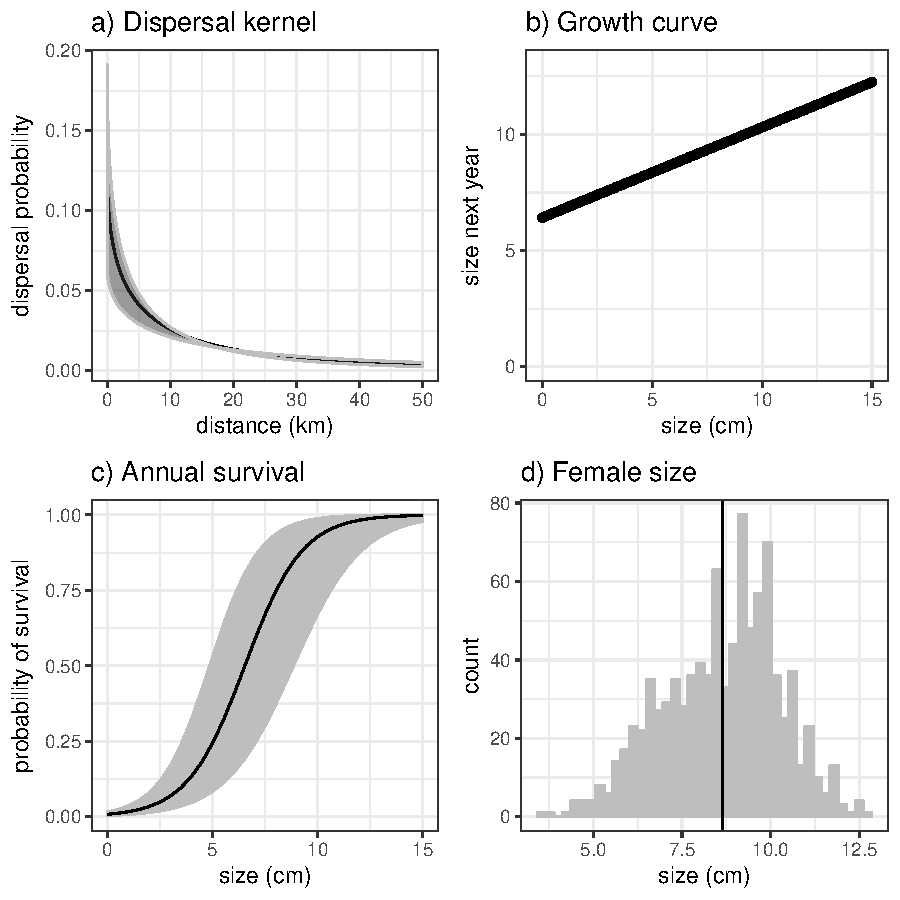
\includegraphics[width = 1.0\textwidth]{\detokenize{../Plots/FigureDrafts/Parameter_inputs.pdf}}
	\caption{WRITE A CAPTION! \label{FIG_ParameterInputs}}
\end{figure}

\begin{figure}[H] % LEP, recruits-per-egg, LRP shown with uncertainty, line for best estimate (using mean offspring size as recruit size)
	\centering
	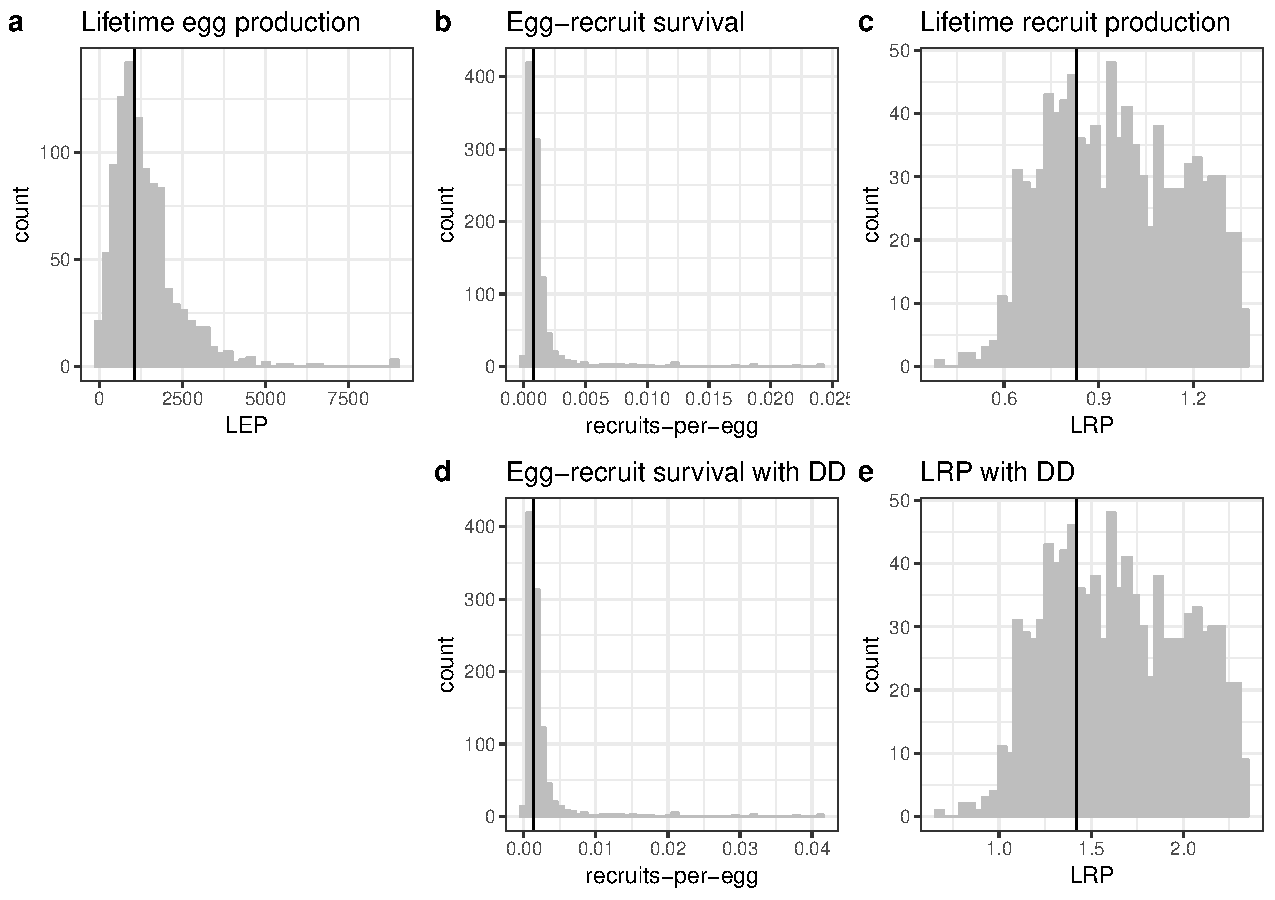
\includegraphics[width = 1.0\textwidth]{\detokenize{../Plots/FigureDrafts/LEP_RperE_LRP.pdf}}
	\caption{Metrics with best estimate (using recruit size of mean of offspring size) and uncertainty. WRITE A CAPTION! \label{FIG_LEP_RperE_LRP}}
\end{figure}

\begin{figure}[H] % SP with line for best estimate (using mean offspring size as recruit size)
	\centering
	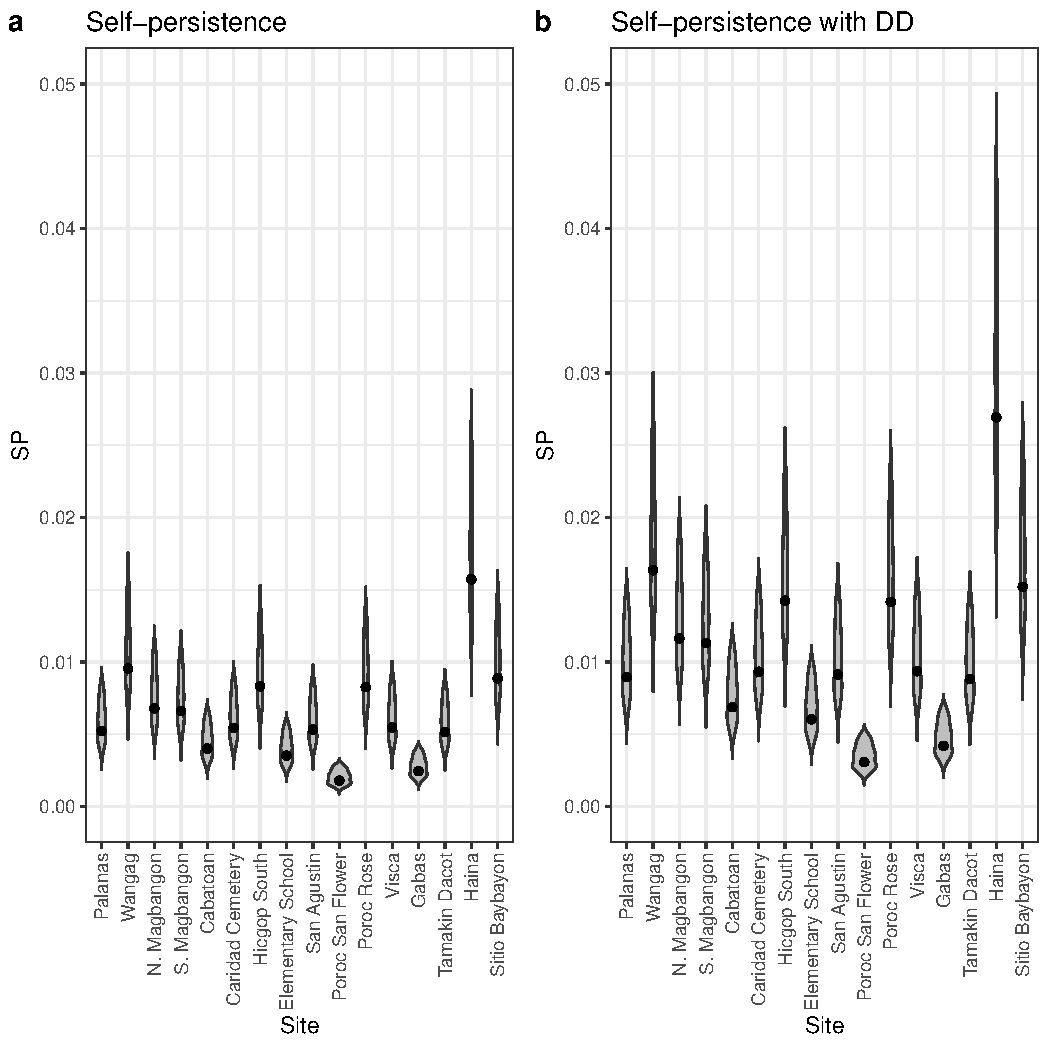
\includegraphics[width = 1.0\textwidth]{\detokenize{../Plots/FigureDrafts/SP_hists_by_site_noSLSTCP.pdf}}
	\caption{Metrics with best estimate (using recruit size of mean of offspring size) and uncertainty. WRITE A CAPTION! \label{FIG_SP}}
\end{figure}

\begin{figure}[H] % NP with line for best estimate (using mean offspring size as recruit size), realized connectivity matrix for best estimate - should re-do without Sitio Lonas, Sitio Tugas, Caridad Proper!
	\centering
	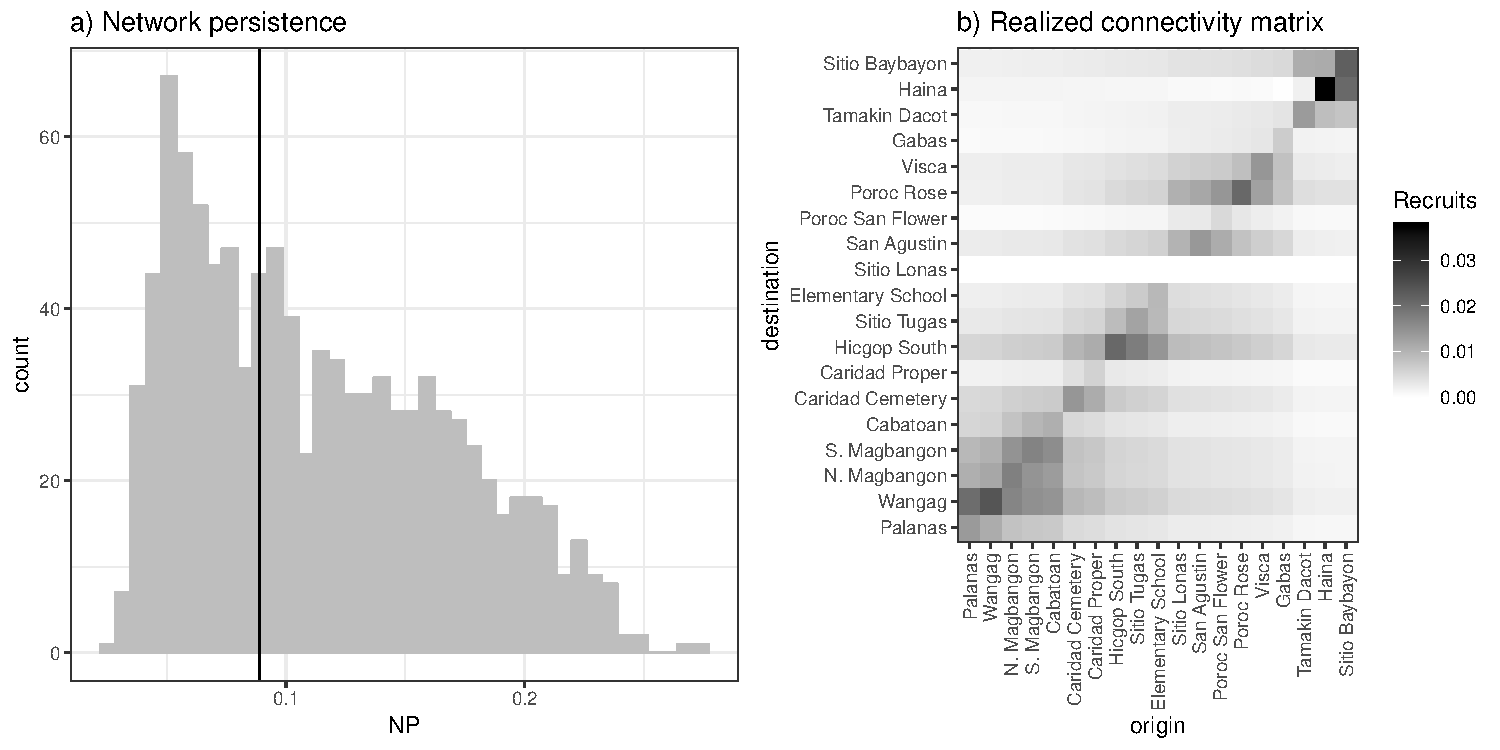
\includegraphics[width = 1.0\textwidth]{\detokenize{../Plots/FigureDrafts/NP_and_connMatrixR.pdf}}
	\caption{Metrics with best estimate (using recruit size of mean of offspring size) and uncertainty. WRITE A CAPTION! \label{FIG_NP_realizedCmat}}
\end{figure}

\begin{figure}[H] % Do we see replacement if we consider all recruits when looking at recuits-per-recruit?
	\centering
	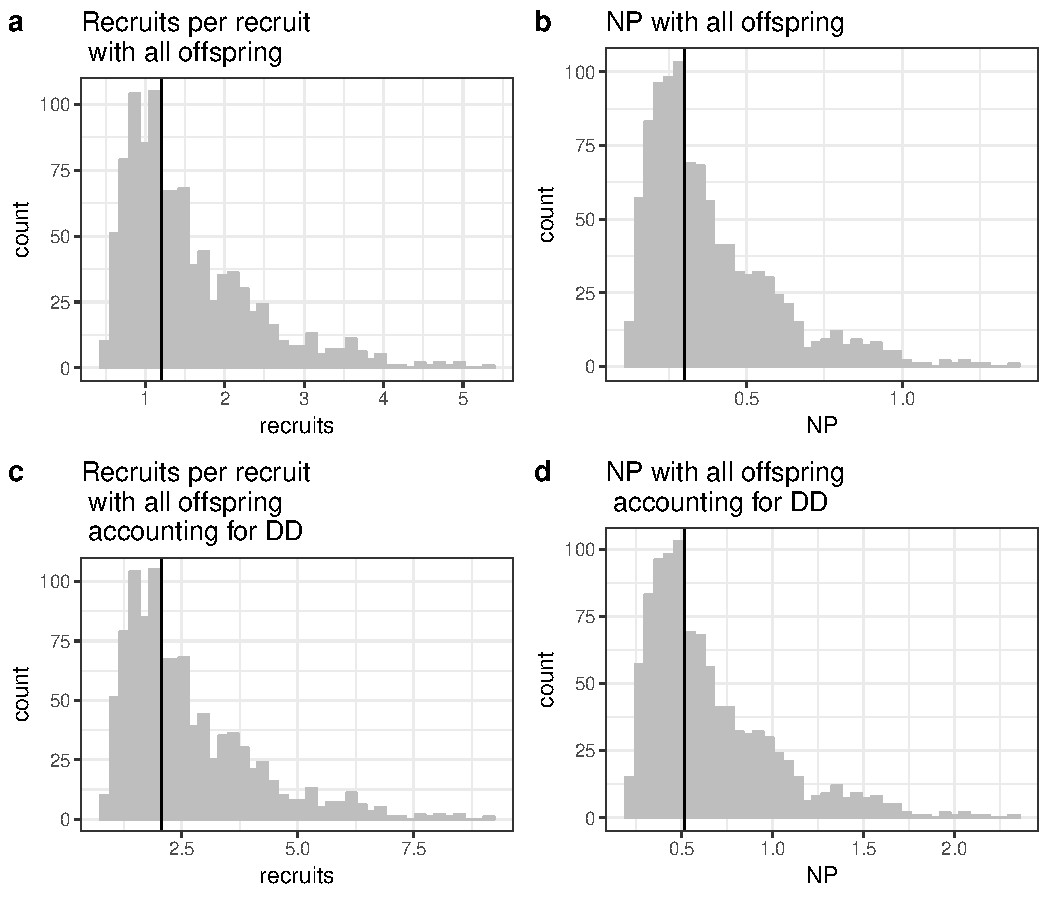
\includegraphics[width = 1.0\textwidth]{\detokenize{../Plots/PersistenceMetrics/Whatifs/LEP_R_and_NP_histograms_whatif_all_offspring.pdf}}
	\caption{Range of parameter inputs for uncertainty runs with all uncertainty included. Census size is the size at fish are considered to have recruited, such that egg-recruit survival ends. Female transition is the size at which fish transition from male to female and their reproductive output is included in the estimate of lifetime egg production (LEP). FINISH LISTING PARAMS! \label{FIG_AllOffspringWhatIf}}
\end{figure}


\section*{Discussion}

previous research suggests 10km dispersal kernel spread for yellowtail clownfish \citep{pinsky2010using}

\newpage{}

{\LARGE Appendix}

\appendix

\renewcommand{\theequation}{A\arabic{equation}}
% redefine the command that creates the equation number.
\renewcommand{\thetable}{A\arabic{table}}
\setcounter{equation}{0}  % reset counter 
\setcounter{figure}{0}
\setcounter{table}{0}
\numberwithin{equation}{section}
\numberwithin{figure}{section}

\section{Uncertainty details}

\subsection{Sensitivity to parameters}

% Range of parameters used as input for uncertainty runs
\begin{figure}[H] % Range of parameter inputs for uncertainty runs
	\centering
	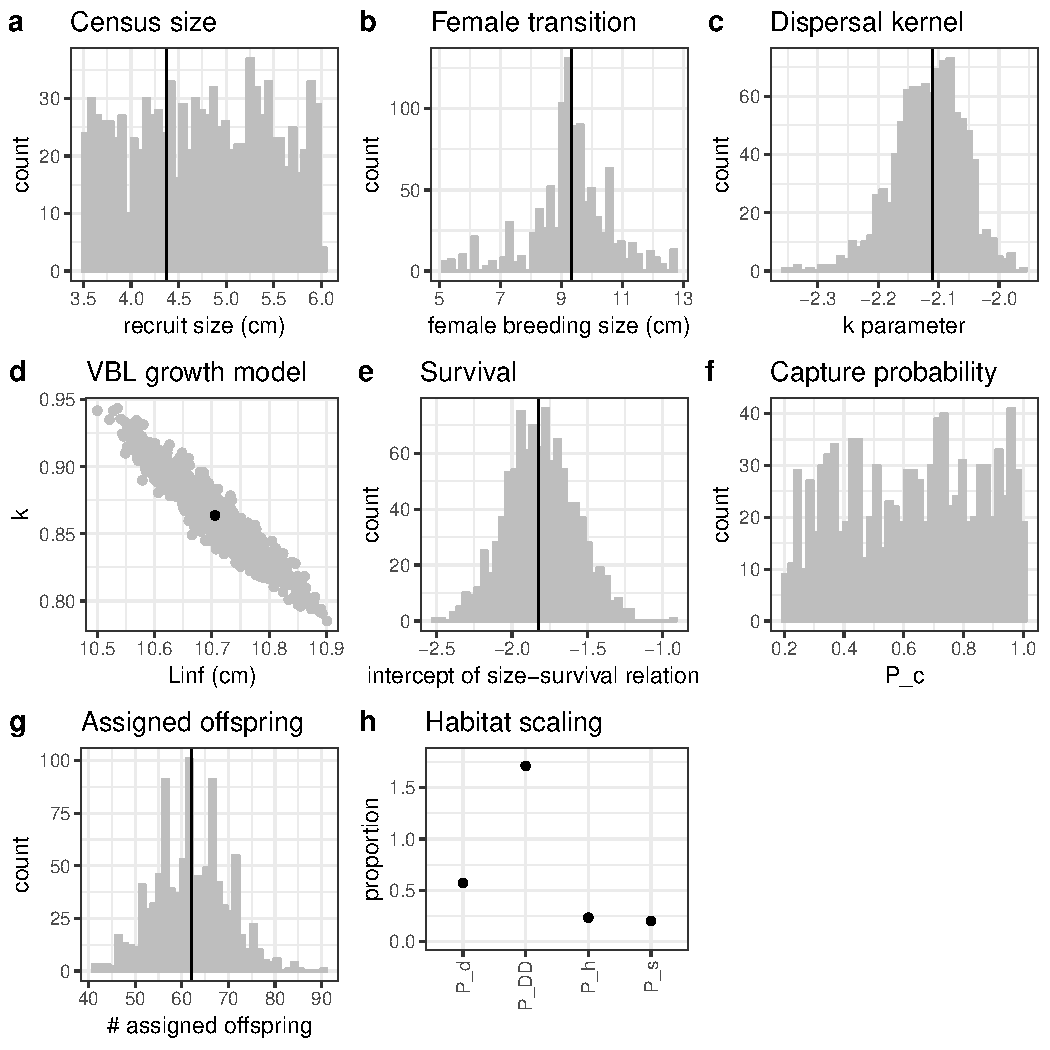
\includegraphics[width = 1.0\textwidth]{\detokenize{../Plots/FigureDrafts/Uncertainty_inputs.pdf}}
	\caption{Range of parameter inputs for uncertainty runs with all uncertainty included. Census size is the size at fish are considered to have recruited, such that egg-recruit survival ends. Female transition is the size at which fish transition from male to female and their reproductive output is included in the estimate of lifetime egg production (LEP). FINISH LISTING PARAMS! \label{APP_FIG_UncertaintyInputs}}
\end{figure}

% Relationships among parameters

\subsection{Effects of different types of uncertainty on metrics}

\begin{figure}[H] % Uncertainty in LEP
	\centering
	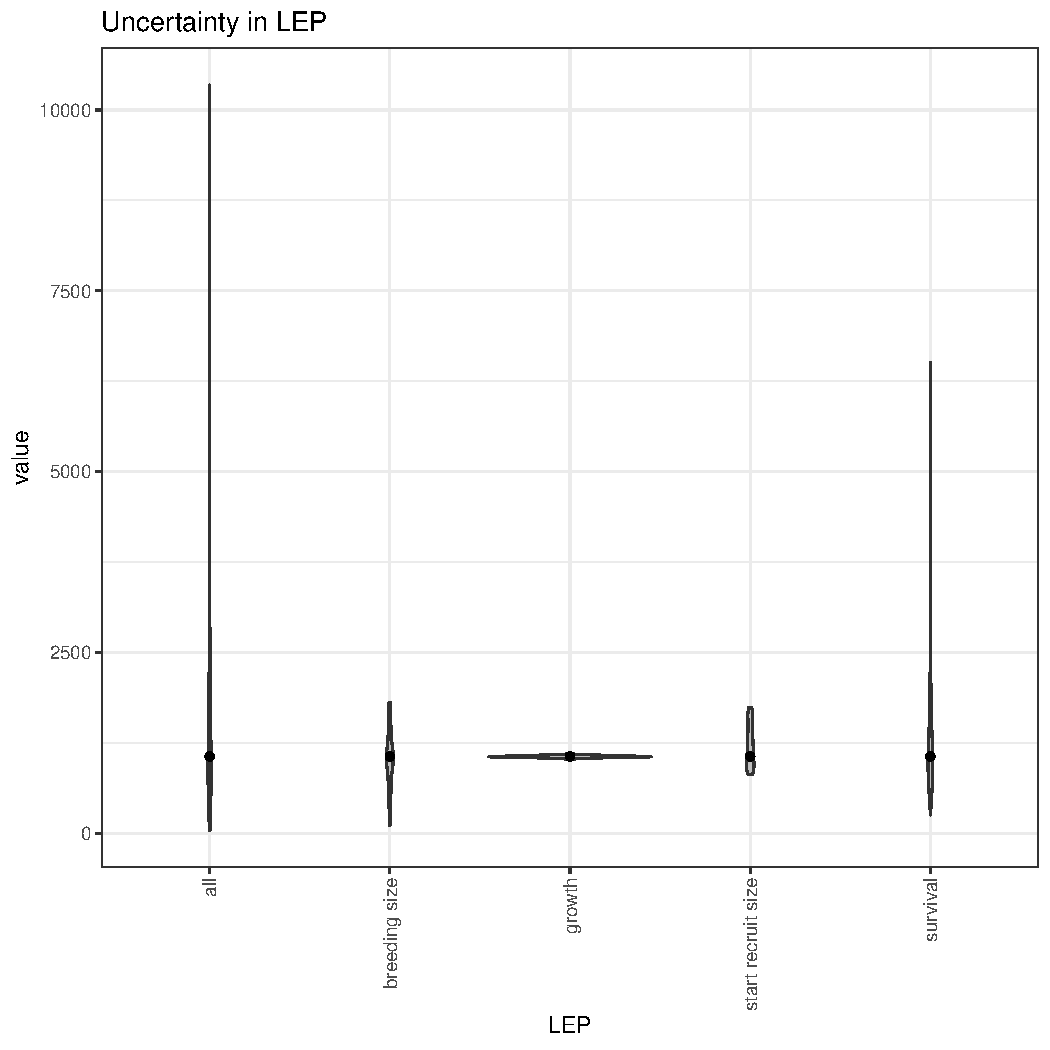
\includegraphics[width = 1.0\textwidth]{\detokenize{../Plots/FigureDrafts/LEP_uncertainty_breakdown.pdf}}
	\caption{WRITE A CAPTION! \label{APP_FIG_Uncertainty_LEP}}
\end{figure}

\begin{figure}[H] % Uncertainty in LEP_R
	\centering
	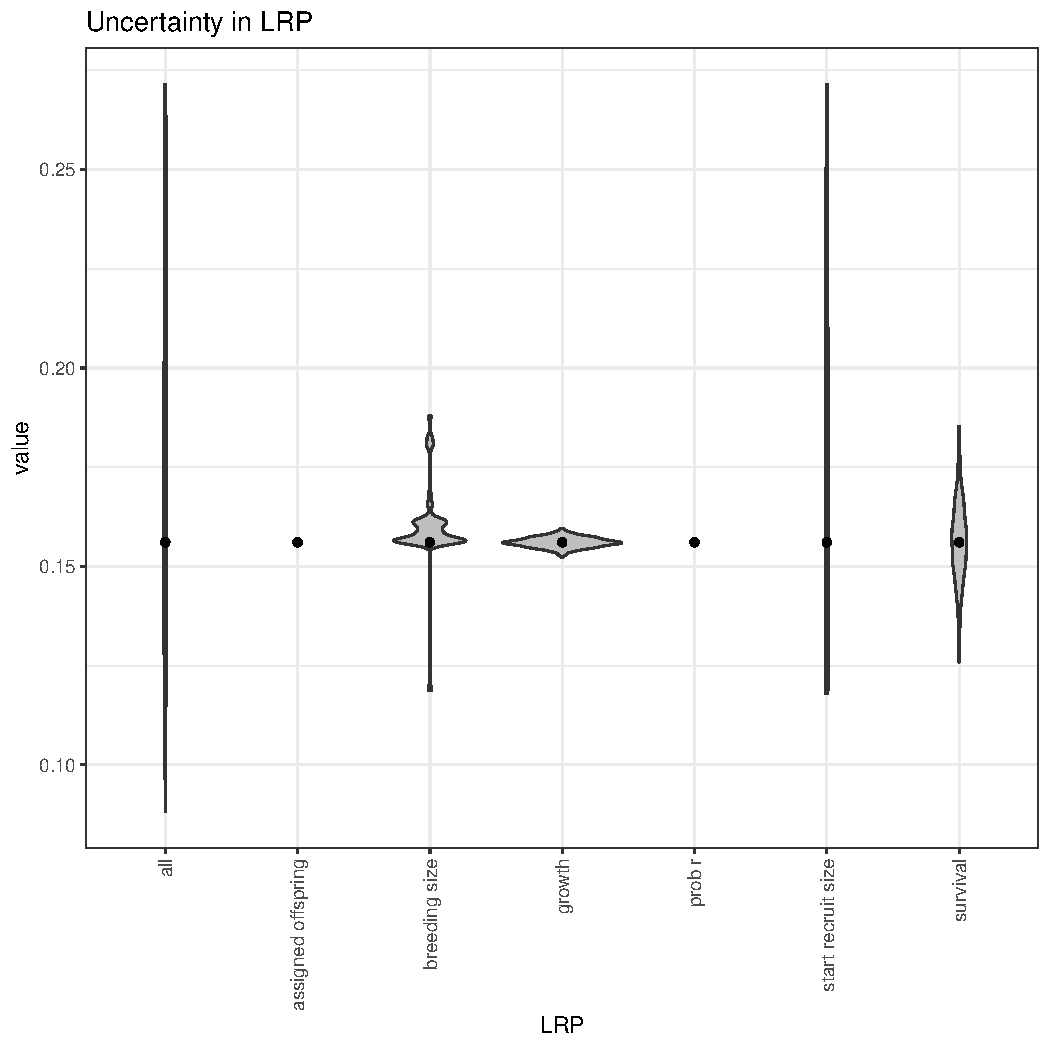
\includegraphics[width = 1.0\textwidth]{\detokenize{../Plots/FigureDrafts/LEP_R_uncertainty_breakdown.pdf}}
	\caption{WRITE A CAPTION! \label{APP_FIG_Uncertainty_LEP_R}}
\end{figure}

\begin{figure}[H] % Uncertainty in recruits-per-egg
	\centering
	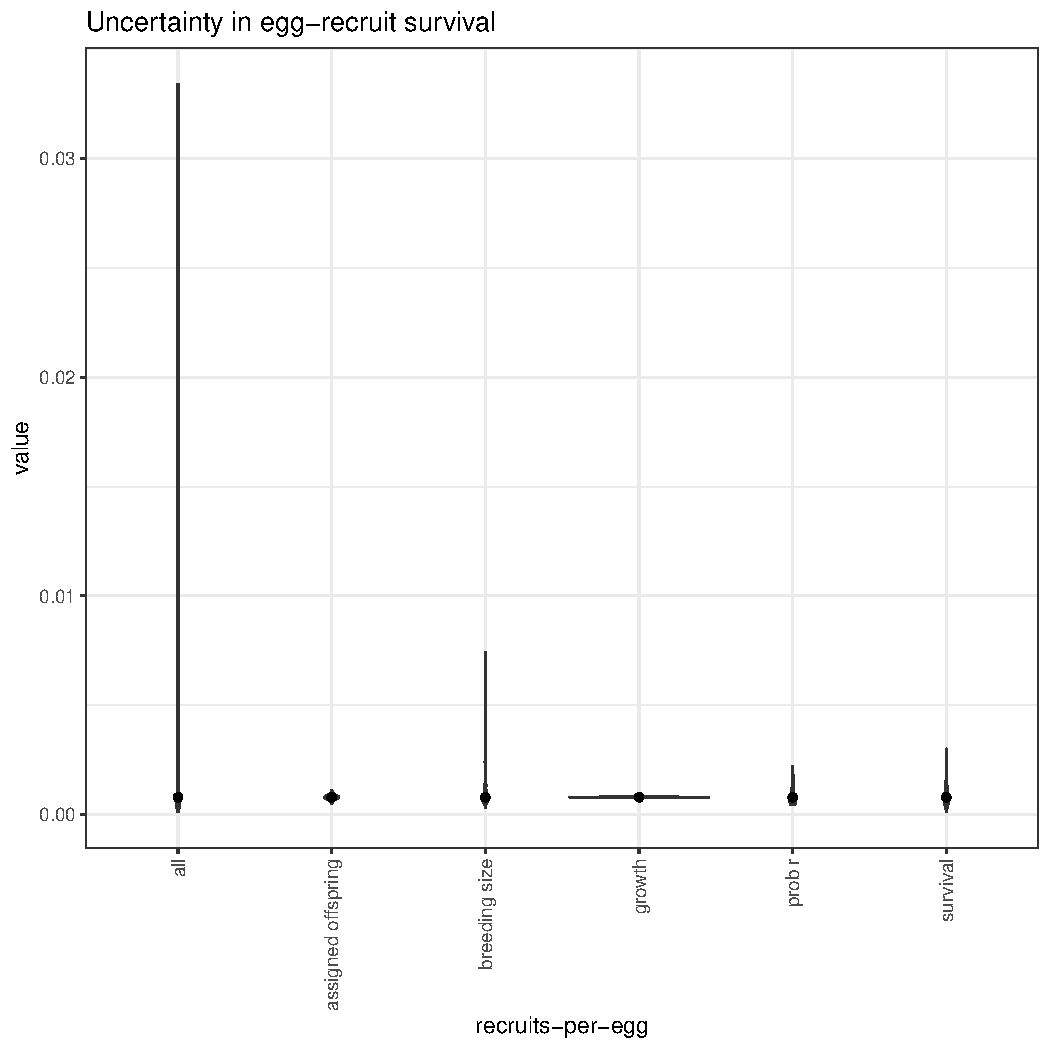
\includegraphics[width = 1.0\textwidth]{\detokenize{../Plots/FigureDrafts/RperE_uncertainty_breakdown.pdf}}
	\caption{WRITE A CAPTION! \label{APP_FIG_Uncertainty_RperE}}
\end{figure}

\begin{figure}[H] % Uncertainty in NP
	\centering
	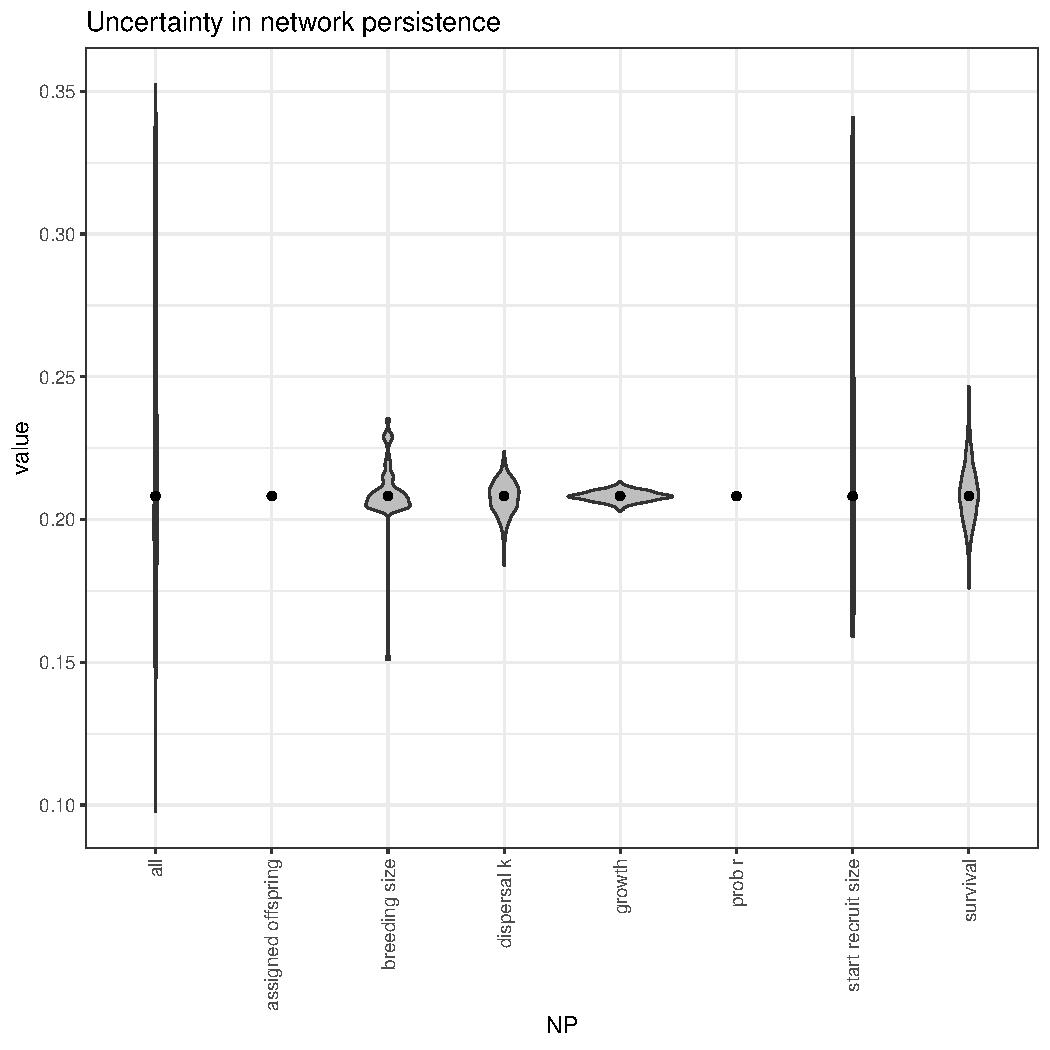
\includegraphics[width = 1.0\textwidth]{\detokenize{../Plots/FigureDrafts/NP_uncertainty_breakdown.pdf}}
	\caption{WRITE A CAPTION! \label{APP_FIG_Uncertainty_NP}}
\end{figure}



\newpage{}

%\bibliography{../../../BibTexReferences}
\bibliography{BibTexReferences}
\bibliographystyle{plainnat}

\end{document}